\chapter{Entropia multivariabile e processi stocastici}

Nel precedente capitolo, abbiamo introdotto il concetto di entropia di una sorgente, vedendo che essa è il limite inferiore del costo di codifica. 
In questo capitolo, approfondiremo il concetto di entropia, analizzandolo più formalmente, introducendo alcune sue proprietà e generalizzandolo a più variabili aleatorie.

\section{Rimandi di teoria della probabilità ed Entropia}

Prima di procedere, facciamo un breve richiamo ad alcuni concetti di teoria della probabilità necessari per la comprensione dei concetti che andremo a trattare in questo capitolo.
Uno \keyword{spazio di probabilità} è una tripla \((\Omega, \mathcal{F}, \Prob)\) dove
\begin{itemize}
  \item \(\Omega\) è un insieme non vuoto, detto spazio dei campioni (o spazio campione);
  \item \(\mathcal{F} \subseteq \mathcal{P}(\Omega)\) è una \(\sigma\)-algebra su \(\Omega\), cioè un insieme di sottoinsiemi di \(\Omega\), incluso lo stesso \(\Omega\), chiuso rispetto all'unione, al complemento e alle unioni numerabili\footnote{$\mathcal{F}$ è: chiuso rispetto all'unione se $\forall A,B \in \mathcal{F}: (A \cup B) \in \mathcal{F}$; chiuso rispetto al complemento se $\forall A \in \mathcal{F}: \bar{A}=(\mathcal{F} \setminus A) \in \mathcal{F}$; chiuso rispetto alle unioni numerabile se $\mathcal{F}$ è infinito numerabile e $\forall \set{A_i}_{i \in \mathbb{N}}: \bigcup_{A \in \set{A_i}}A \in \mathcal{F}$.};
  \item \(\Prob: \mathcal{F} \to [0,1]\) è una misura di probabilità, cioè una funzione tale che \(\Prob[\Omega] = 1, \Prob[\emptyset] = 0\) e che è \(\sigma\)-additiva, ovvero per ogni famiglia numerabile di eventi disgiunti \({\{A_i\}}_{i \in \mathbb{N}} \subseteq \mathcal{F}\) si ha che
  \[\Prob\left[\bigcup_{i=1}^{\infty} A_i\right] = \sum_{i=1}^{\infty} \Prob[A_i]\]
\end{itemize}

Una \keyword{variabile aleatoria discreta} su uno spazio di probabilità \((\Omega, \mathcal{F}, \Prob)\) è un applicazione misurabile \(S: \Omega \to \SCal\), dove \(\SCal\) è un insieme discreto (finito o numerabile), che ad un evento in $\Omega$ associa un simbolo in $\SCal$.

Essendo \(S\) misurabile, è possibile associare una funzione \q{massa} di probabilità (distribuzione su \(\SCal\)) \(p: \SCal \to [0,1]\) definita come \(p(s) = \Prob[S=s] = \Prob[S^{-1}(s)]\)\footnote{La notazione $\Prob[X=x]$ risulta spesso comoda, ma è abusiva: la notazione formalmente corretta è $\Prob[S^{-1}(s)]$ poiché $\Prob$ è definita su $\mathcal{F}$ e $S^{-1}(s) \in \mathcal{F}$.}.
Per chiarezza e semplicità, assumeremo che la variabile $A$ abbia alfabeto $\mathcal{A}$, che $B$ abbia alfabeto $\mathcal{B}$ e così via.

\begin{definition}{Entropia di una variabile aleatoria}
  Sia \(X\) variabile aleatoria discreta con distribuzione di probabilità \(p\).
  L'\keyword{entropia} di \(X\) è definita come
  \[H(X) = -\sum_{x \in \mathcal{X}} p(x) \log( p(x))= \EV{\log(\frac{1}{p(x)})}\]
\end{definition}

A seguito del teorema di Shannon (\Cref{thm:shannon}), possiamo interpretare questa quantità come il limite inferiore del costo di codifica per una sorgente binaria.
Dunque possiamo vedere l'entropia come la più corta descrizione binaria del valore di \(X\), o in altre parole il numero medio di domande binarie necessarie per identificare il valore di \(X\). Insomma, $H(X)$ rappresenta il grado di incertezza sul valore emesso da $X$.

\begin{definition}{Definizione assiomatica dell'entropia di Shannon}
  Sia \({(H_m)}_{m \geq 1}\) una famiglia di funzioni, di cui ogni \(H_m \in {(H_m)}_{m \geq 1}\) è una funzione a \(m\) variabili con le seguenti proprietà:
  \begin{description}
    \item[simmetria]: \(\forall \sigma \in S_m: H_m(p_1,\ldots,p_m) = H_m(p_{\sigma(1)},\ldots,p_{\sigma(m)})\), con \( S_m\) insieme delle permutazioni di \(\set{1,\ldots,m}\). In altre parole, l'entropia non dipende dall'ordine in cui i simboli appaiono nell'alfabeto, ma solo dalla distribuzione $p$.
    \item[normalizzazione]: \(H_2\left(\frac{1}{2}, \frac{1}{2}\right) = 1\).
    \item[continuità]: \(H_2(p,1-p)\) funzione continua di \(p\).
    \item[raggruppamento]:
    \[H_m(p_1,p_2,p_3,\ldots,p_m) = H_{m-1}(p_1 + p_2,p_3,\ldots,p_m)+(p_1+p_2)H_2\left(\frac{p_1}{p_1+p_2},\frac{p_2}{p_1+p_2}\right)\]
  \end{description}
\end{definition}

Presa questa definizione, si vede che l'unica implementazione possibile per l'entropia è \[H_m(p_1,\ldots,p_m) = - \sum_{i=1}^{m} p_i \log(p_i)\] preso un qualsiasi \(m\geq 1\).

A questo punto, introduciamo il concetto di variabile aleatoria multipla ed estendiamo l'entropia a tale caso.

\begin{definition}{Entropia Congiunta}
  Siano \(X, Y\) variabili aleatorie. Definiamo la \keyword{variabile aleatoria congiunta}, rappresentata dalla coppia \((X,Y)\), come:
  \[(X,Y): \omega \in \Omega \mapsto (X(\omega), Y(\omega)) \in \mathcal{X} \times \mathcal{Y}\]
  
  La cui funzione di massa di probabilità congiunta è data da
  \[p(x,y) = \Prob[X=x, Y=y] = \Prob[X=x \land Y=y] = \Prob[X^{-1}(x) \cap Y^{-1}(y)]\]
  L'\keyword{entropia congiunta} di \(X\) e \(Y\) è definita come
  \[H(X,Y) = - \sum_{\substack{x \in \mathcal{X},\\ y \in \mathcal{Y}}} p(x,y) \log(p(x,y)) = \EV{\log\left(\frac{1}{p(x,y)}\right)}\]
\end{definition}

\begin{definition}{Condizionamento}
  Dati \(A,B \subseteq \Omega\), definiamo \(A|B\) l'evento \(A\) condizionato da \(B\) (\qi{A dato B}) come l'evento tale che
  \[\Prob[A|B] = \frac{\Prob[A \cap B]}{\Prob[B]}\]

  In particolare, se \(X,Y\) sono variabili aleatorie, definiamo \(p(y|x) = \Prob[Y=y|X=x]\)

  Si ha dunque che \(\forall x \in \mathcal{X}, y \in \mathcal{Y}, p(y|x) = \frac{p(x,y)}{p(x)}\), cioè \(p(x,y) = p(x)p(y|x)\).
\end{definition}

Possiamo notare che  \(\forall x \in \mathcal{X}\) fissato, \(p(y|x)\) è una distribuzione di probabilità su \(\mathcal{Y}\).
Infatti,\footnote{Date \(X,Y\) variabili aleatorie, si ha che \(\sum_{y \in \mathcal{Y}} p(x,y) = p(x), \forall x \in \mathcal{X}\) per la proprietà di marginalizzazione di una funzioni di massa di probabilità congiunta.
In altre parole, data una funzione di massa di probabilità congiunta \(p(x,y)\), è sempre possibile ricavare le distribuzioni marginali $p(x)$ e $p(y)$. L'operazione inversa è possibile solo quando $X$ e $Y$ sono indipendenti, ovvero quando si osserva $p(x,y)=p(x)p(y)$.}
\[\sum_{y \in \mathcal{Y}} p(y|x) = \sum_{y \in \mathcal{Y}} \frac{p(x,y)}{p(x)} = \frac{1}{p(x)} \sum_{y \in \mathcal{Y}} p(x,y) = \frac{p(x)}{p(x)} = 1\]

Possiamo vedere $p(y|x)$ come funzione massa di probabilità di una variabile aleatoria \(Y|X=x\).

\begin{definition}{Entropia Condizionata}
  Siano \(X,Y\) variabili aleatorie.
  L'\keyword{entropia condizionata} di \(Y|X\) è definita come
  \[H(Y|X) = \sum_{x \in \mathcal{X}} p(x) H(Y|X=x) = - \sum_{x \in \mathcal{X}} p(x) \sum_{y \in \mathcal{Y}} p(y|x) \log(p(y|x)) = \]
  \[= -\sum_{\substack{x \in \mathcal{X}\\y \in \mathcal{Y}}} p(x,y) \log (p(y|x)) = \EV{\log\left(\frac{1}{p(y|x)}\right)}[x,y]\]
  
  ovvero la media delle entropie di \(Y|X=x\) al variare di \(x\), pesata secondo la probabilità \(p(x)\).
\end{definition}

Definite queste quantità, vediamo come si relazionano tra di loro, partendo dalla prima regola di catena.

\begin{proposition}{Regola di catena}
  Date \(X,Y\) variabili aleatorie, si ha che
  \[H(X,Y) = H(X) + H(Y|X)\]
\end{proposition}

\begin{proof}
  \[H(X,Y) =-\sum_{\substack{x \in \mathcal{X},\\ y \in \mathcal{Y}}} p(x,y) \log(p(x,y)) = -\sum_{\substack{x \in \mathcal{X},\\ y \in \mathcal{Y}}} p(x,y) \log(p(x)p(y|x)) = \]
  \[= - \sum_{\substack{x \in \mathcal{X},\\ y \in \mathcal{Y}}} p(x,y)\left(\log(p(x)) + \log(p(y|x))\right)  = - \sum_{\substack{x \in \mathcal{X},\\ y \in \mathcal{Y}}} p(x,y) \log(p(x)) - \sum_{\substack{x \in \mathcal{X},\\ y \in \mathcal{Y}}} p(x,y) \log(p(y|x)) =\]
  \[=- \sum_{x \in \mathcal{X}} \log(p(x))\sum_{y \in \mathcal{Y}} p(x,y)  - \sum_{\substack{x \in \mathcal{X},\\ y \in \mathcal{Y}}} p(x,y) \log(p(y|x)) = H(X) + H(Y|X)\]
\end{proof}

\begin{example}{}
  Prendiamo in considerazione due variabili aleatorie quaternarie \(X,Y\) la cui probabilità congiunta è data dalla seguente tabella:
  \begin{center}
    \begin{tabular}{c|c c c c}
      \(Y \backslash X\) & \(a\) & \(b\) & \(c\) & \(d\) \\
      \hline
      \(1\) & \(\frac{1}{8}\) & \(\frac{1}{16}\) & \(\frac{1}{32}\) & \(\frac{1}{32}\) \\
      \(2\) & \(\frac{1}{16}\) & \(\frac{1}{8}\) & \(\frac{1}{32}\) & \(\frac{1}{32}\) \\
      \(3\) & \(\frac{1}{16}\) & \(\frac{1}{16}\) & \(\frac{1}{16}\) & \(\frac{1}{16}\) \\
      \(4\) & \(\frac{1}{4}\) & \(0\) & \(0\) & \(0\) \\
    \end{tabular}
  \end{center}

  Verifichiamo che \(H(X) = \frac{7}{4}\).
  Per calcolare l'entropia di \(X\), dobbiamo prima calcolare la distribuzione di probabilità marginale di \(X\):
  \begin{itemize}
    \item \(p(a) = \frac{1}{8} + \frac{1}{16} + \frac{1}{16} + \frac{1}{4} = \frac{1}{2}\)
    \item \(p(b) = \frac{1}{16} + \frac{1}{8} + \frac{1}{16} + 0 = \frac{1}{4}\)
    \item \(p(c) = \frac{1}{32} + \frac{1}{32} + \frac{1}{16} + 0 = \frac{1}{8}\)
    \item \(p(d) = \frac{1}{32} + \frac{1}{32} + \frac{1}{16} + 0 = \frac{1}{8}\)
  \end{itemize}
  Abbiamo dunque che
  \[H(X) = \frac{1}{2}\log(2)+\frac{1}{4}\log(4)+\frac{1}{8}\log(8)+\frac{1}{8}\log(8) = \]
  \[= \frac{1}{2}+\frac{1}{4}\cdot 2 + \frac{2}{8} \cdot 3 = \frac{7}{4}\]
  
  Verifichiamo ora che \(H(Y) = 2\).
  Analogamente a prima, calcoliamo la distribuzione di probabilità marginale di \(Y\):
  \begin{itemize}
    \item \(p(1) = \frac{1}{8} + \frac{1}{16} + \frac{1}{32} + \frac{1}{32} = \frac{1}{4}\)
    \item \(p(2) = \frac{1}{16} + \frac{1}{8} + \frac{1}{32} + \frac{1}{32} = \frac{1}{4}\)
    \item \(p(3) = \frac{1}{16} + \frac{1}{16} + \frac{1}{16} + \frac{1}{16} = \frac{1}{4}\)
    \item \(p(4) = \frac{1}{4} + 0 + 0 + 0 = \frac{1}{4}\)
  \end{itemize}
  Dunque
  \[H(Y) = 4 \cdot \frac{1}{4} \log(4) = 2\]

  Verifichiamo ora che \(H(X,Y) = \frac{27}{8}\).
  In questo caso è sufficiente calcolare direttamente l'entropia congiunta:
  \[H(X,Y) = 2\cdot\frac{1}{8}\cdot 3 + 6\cdot\frac{1}{16}\cdot 4 + \frac{1}{4}\cdot 2 + 4 \cdot \frac{1}{32}\cdot 5= \]
  \[= \frac{6}{8} + \frac{24}{16} + \frac{2}{4} + \frac{20}{32} = \frac{27}{8}\]
  

  Infine, si ha che \(H(X|Y) = H(X,Y)-H(X) = \frac{27}{8} - \frac{7}{4} = \frac{13}{8}\) e che \(H(Y|X) = H(X,Y)-H(Y) = \frac{27}{8} - 2 = \frac{11}{8}\).
\end{example}

Dall'esempio precedente, possiamo osservare che l'entropia congiunta è simmetrica rispetto alle variabili coinvolte, mentre l'entropia condizionata no.
In generale, \(H(X|Y) \neq H(Y|X)\) e \(H(X,Y) = H(Y,X)\).

Tuttavia, la regola di catena ci assicura che
\[H(Y)+H(X|Y)=H(Y,X)=H(X,Y) = H(X)+H(Y|X)\]
ovvero
\[H(Y) - H(Y|X) = H(X) - H(X|Y)\]

Possiamo generalizzare questo risultato a più variabili aleatorie.

\begin{proposition}{Regola di catena con condizionamento}
  Date \(X,Y,Z\) variabili aleatorie, si ha che
  \[H(X,Y|Z) = H(X|Z) + H(Y|X,Z)\]
  ossia
  \[- \sum_{\substack{x \in \mathcal{X},\\y\in\mathcal{Y},\\z \in \mathcal{Z}}} p(x,y,z) \log(p(x,y|z)) = -\sum_{\substack{x\in\mathcal{X},\\z\in\mathcal{Z}}} p(x,z)\log(p(x|z)) - \sum_{\substack{x \in \mathcal{X},\\y \in \mathcal{Y},\\z \in \mathcal{Z}}} p(x,y,z) \log(p(y|x,z))\]
\end{proposition}


\begin{definition}{Divergenza di Kullback-Leibler (entropia relativa)}
  Siano \(p,q\) due distribuzioni di probabilità su uno stesso insieme discreto \(\mathcal{X}\).
  La \keyword{divergenza di Kullback-Leibler} tra \(p\) e \(q\) è definita come
  \[D_{KL}(p ||q) = \sum_{x \in \mathcal{X}} p(x) \log\left(\frac{p(x)}{q(x)}\right) \]
\end{definition}

\begin{note}{}
  Essendo che possono esistere \(x\) tali che \(q(x) = 0\) e \(p(x) > 0\), la divergenza di Kullback-Leibler può essere infinita.
\end{note}

La divergenza di Kullback-Leibler è spesso interpretata come una distanza, anche se non ne rispetta propriamente le proprietà matematiche.

Infatti non sono soddisfatte la simmetria, \(D(p||q) \neq D(q||p)\), e la disuguaglianza triangolare.
La divergenza di Kullback-Leibler è però \textit{definita positiva}, ovvero \(D_{KL}(p||q) \geq 0\) con uguaglianza se e solo se \(p=q\).\footnote{Questo segue in maniera diretta dall'\Cref{eq:gibbs} vista in precedenza}

\begin{definition}{Mutua Informazione}
  Siano \(X,Y\) variabili aleatorie congiunte.
  La \keyword{mutua informazione} tra \(X\) e \(Y\) è definita come
  \[I(X;Y) = D_{KL}(p(x,y) || p(x)p(y)) = \sum_{\substack{x \in \mathcal{X}\\y \in \mathcal{Y}}} p(x,y) \log\left(\frac{p(x,y)}{p(x)p(y)}\right)\]

  Essendo che \(p(x,y)=p(x)p(y), \forall x\in\mathcal{X}, y\in\mathcal{Y} \iff\) \(X\) e \(Y\) sono indipendenti, si ha che \(I(X;Y) = 0 \iff\) \(X\) e \(Y\) sono indipendenti.
\end{definition}

Intuitivamente, la mutua informazione misura la quantità di informazione, come riduzione di incertezza, che una variabile aleatoria fornisce sull'altra.
Questa è ovviamente nulla quando le due variabili sono indipendenti.

Si ha inoltre che
\[I(X;Y) = \sum_{\substack{x \in \mathcal{X}\\y \in \mathcal{Y}}} p(x,y) \log\left(\frac{p(x,y)}{p(x)p(y)}\right) = \]
\[= \sum_{\substack{x \in \mathcal{X}\\y \in \mathcal{Y}}} p(x,y) \log\left(\frac{p(y|x)}{p(y)}\right) = \sum_{\substack{x\in\mathcal{X}\\y\in\mathcal{Y}}}p(x,y)\log(p(y|x)) - \sum_{y\in\mathcal{Y}}\log(p(y))\sum_{x\in\mathcal{X}}p(x,y)\]
\[= H(Y)-H(Y|X)\]


Un modo intuitivo per visualizzare le relazioni tra le varie quantità di informazione viste finora è tramite i diagrammi di Venn modificati come in \Cref{fig:venn_info}.

\begin{figure}[H]
  \centering
  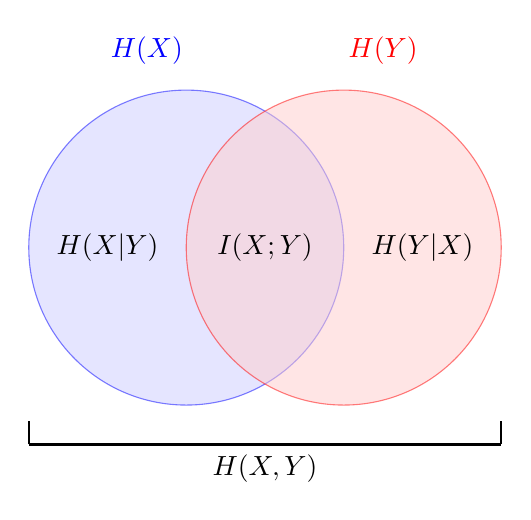
\begin{tikzpicture}
    \def \r {2} % radius of circles
    \def \d {2} % distance between centers

    % Draw circles
    \draw[fill=blue!20, draw=blue, opacity=0.5] (-\d/2,0) circle (\r);
    \draw[fill=red!20, draw=red, opacity=0.5] (\d/2,0) circle (\r);

    % Labels
    \node at (-\d/2-0.5, \r + 0.5) [blue] {\(H(X)\)};
    \node at (\d/2+0.5, \r + 0.5) [red] {\(H(Y)\)};
    \node at (0,0) {\(I(X;Y)\)};
    \node at (-\d, 0) {\(H(X|Y)\)};
    \node at (\d, 0) {\(H(Y|X)\)};

    \draw[thick] (-\d/2-\r,-\r-0.5) to node[midway, below, ] {\(H(X,Y)\)} (\d/2+\r,-\r-0.5);
    \draw[thick] (-\d/2-\r,-\r-0.5) -- ++(0,0.3);
    \draw[thick] (\d/2+\r,-\r-0.5) -- ++(0,0.3);
  \end{tikzpicture}
  \caption{Diagramma di Venn per le quantità di informazione.}\label{fig:venn_info}
\end{figure}

\begin{definition}{Informazione mutua condizionata}
  Date \(X,Y,Z\) variabili aleatorie, la \keyword{mutua informazione condizionata} tra \(X\) e \(Y\) dato \(Z\) è definita come
  \[I(X;Y|Z) = H(X|Z) - H(X|Y,Z)\]
\end{definition}

Possiamo dunque generalizzare le regole di catena a \(n\) variabili.

\begin{proposition}{}
  Siano \(X_1, X_2, \ldots, X_n, Y\) variabili aleatorie.
  Si ha che
  \[H(X_1, X_2, \ldots, X_n) = H(X_1) + H(X_2|X_1) + \cdots + H(X_n | X_1, X_2, \ldots, X_{n-1}) = \]
  \[=H(X_1) + \sum_{i=2}^{n} H(X_i | X_{i-1}, \ldots, X_1)\]
  E che
  \[I(X_1, \ldots, X_n; Y) = I(X_1; Y) + I(X_2; Y | X_1) + \cdots + I(X_n; Y | X_1, \ldots, X_{n-1}) = \]
  \[=I(X_1;Y) + \sum_{i=2}^{n} I(X_i; Y | X_{i-1}, \ldots, X_1)\]
\end{proposition}

\subsection{Limiti dell'informazione mutua}\label{subs:mutual_information_limits}

Essendo \(I\) definita in termini di divergenza di Kullback-Leibler, \(I\) è definita positiva, dunque \(I(X;Y) \geq 0\) e l'uguaglianza si verifica se e solo se \(X\) e \(Y\) sono indipendenti.
In tal caso infatti, le due variabili non forniscono alcuna informazione l'una sull'altra.

Da un punto di vista formale, questo si ha perché \(p(x,y)=p(x)p(y)\) per ogni \(x \in \mathcal{X}\) e \(y \in \mathcal{Y}\) se e solo se \(X\) e \(Y\) sono indipendenti.

Poiché \(I(X;Y) = H(X) - H(X|Y)\) e l'entropia è una quantità non negativa, $I$ è massima quando $H(X|Y)=0$. Ciò si verifica quando l'incertezza sull'emissione di $X$ è nulla dopo aver osservato l'emissione di $Y$, ovvero quando $X$ è deterministicamente ricavato da $Y$, ovvero: \footnote{Ricordiamo che dati due insiemi \(A,B\), con \(B^A\) si intende l'insieme delle funzioni da \(A\) a \(B\), come visto nel primo capitolo.}
\[\exists f \in \mathcal{X}^\mathcal{Y} \st X= f\circ Y\]

In tal caso, si ha che \(I(X;Y) = H(X)\).
In particolare, per \(f = id\) si ha che \(I(X;X) = H(X)\), giustificando il significato intuitivo dato all'entropia nel capitolo precedente come misura dell'autoinformazione di una variabile aleatoria.

Infine, notiamo che
\[I(X;Y)\geq 0 \implies H(X) \geq H(X|Y)\]
cioè che \qi{il condizionamento non aumenta l'entropia}. Infatti, intuitivamente, la conoscenza di $Y$ può togliere incertezza dall'emissione di $X$, ma di certo non può aggiungerla. Per questo motivo, si osserva il seguente risultato.

\begin{proposition}{}
  Date \(X_1, X_2, \ldots, X_n\) variabili aleatorie, si ha che
  \(H(X_1, \ldots, X_n)\leq \sum_{i=1}^n H(X_i)\)
\end{proposition}
\begin{proof}
  Si ha
  \[H(X_1, \ldots, X_n) = H(X_1) + \sum_{i=2}^{n}H(X_i|X_{i-1}, \ldots, X_1)\leq \sum_{i=1}^n H(X_i)\]
  poiché \(H(X_i|X_{i-1}, \ldots, X_1) \leq H(X_i)\) per ogni \(i=2,\ldots,n\).
\end{proof}

\section{Catene di Markov e Processi Stocastici}

\begin{definition}{Catena di Markov (3 variabili)}
  Date tre variabili aleatorie \(X, Y, Z\) si dice che formano una \keyword{catena di Markov} in quest'ordine, denotato come \(X \to Y \to Z\) se vale che
  \[\forall x \in X, y \in Y, z \in Z, p(x,y,z) = p(x)p(y|x)p(z|y)\]
\end{definition}

\begin{observation}{}
  Ciò che cambia rispetto alla definizione generale di variabili aleatorie è che \(p(z|x,y) = p(z|y)\), ovvero che \(Z\) è condizionatamente indipendente da \(X\) dato \(Y\),
  ovvero \(p(x,z|y) = p(x|y)p(z|y)\). 
  
  Si ha infatti che in generale 
  \[p(x,z|y) = \frac{p(x,y,z)}{p(y)} = \frac{p(x,y)p(z|x,y)}{p(y)} = p(x|y)p(z|x,y) \]
  e dunque si ha che \(p(z|x,y) = p(z|y)\) se e solo se \(X\) e \(Z\) sono condizionatamente indipendenti dato \(Y\).
\end{observation}

\begin{proposition}[label=prop:markov_chain_third_funcion_second]{}
  Siano \(Y,Z\) variabili aleatorie tali che \(Z = f \circ Y\) per qualche funzione \(f \in \mathcal{Z}^{\mathcal{Y}}\), allora \( \forall X\) variabile aleatoria, \(X \to Y \to Z\).
\end{proposition}
\begin{proof}
  Si ha per ipotesi che
  \begin{equation*}
    p(z|y) = \begin{cases}
      1 & \text{se } z = f(y) \\
      0 & \text{altrimenti}
    \end{cases}
  \end{equation*}
  Allora se \(z\neq f(y)\), \(0= p(z|y)=\sum_{x\in\mathcal{X}}p(x,z|y)\).
  
  Essendo che \(p(x,z|y)\geq 0\), \(\forall x \in \mathcal{X}\), si ha che \(\sum_{x\in\mathcal{X}}p(x,z|y) \iff p(x,z|y)=0 \; \forall x\), e dunque \(0=p(x,z|y) = p(x|y)p(z|y) = p(x|y)\cdot 0\).

  Se invece \(z = f(y)\), allora \(\sum_{z' \in \mathcal{Z}}p(x,z'|y)=p(x,z|y)\) poiché, per \(z'\neq z\), \( p(x,z'|y)=p(z|y)p(x|z,y)=0 \cdot p(x|z,y)\). 
  Ma stando sommando su tutti gli elementi di \(\mathcal{Z}\), si ha che 
  \[\sum_{z' \in \mathcal{Z}}p(x,z'|y) = p(x|y)=p(x|y)\cdot 1 = p(x|y)p(z|y)\]
  Dunque
  \[p(x,z|y) = \sum_{z' \in \mathcal{Z}}p(x,z'|y)= p(x|y)p(z|y)\]
\end{proof}

\begin{proposition}[label=prop:dpi]{Disuguaglianza di Data Processing (DPI)}
  Date \(X,Y,Z\) variabili aleatorie.
  Se \(X \to Y \to Z\) allora \(I(X;Y) \geq I(X;Z)\).

  Inoltre, vale l'uguaglianza se e solo se \(X \to Z \to Y\).
\end{proposition}

\begin{observation}{}
  Questa disuguaglianza ci dice che (nel caso particolare di \(Z = f \circ Y\)), non si può \qi{elaborare} il dato \(Y\) per ottenere più informazioni su \(X\) rispetto a quelle che già si avevano in \(Y\).
\end{observation}

\begin{proof}
  Per la regola di catena,
  \[I(X;Y)+I(X;Z|Y)=I(X;Y,Z) = I(X;Z) + I(X;Y|Z)\]
  Se \(X \to Y \to Z\), abbiamo che \(X\) e \(Z\) sono condizionatamente indipendenti dato \(Y\), dunque \(I(X;Z|Y)=0\) dalla \Cref{subs:mutual_information_limits}
  Allora
  \[I(X;Y) = I(X;Z) + I(X;Y|Z) \]
  Essendo che \(I(X;Y|Z) \geq 0\), si ha la tesi.

  Inoltre, vale l'uguaglianza se e solo se \(I(X;Y|Z)=0\), ovvero se e solo se \(X\) e \(Y\) sono condizionatamente indipendenti dato \(Z\), ovvero \(X\to Z \to Y\).
\end{proof}

È importante notare che l'equazione ricavata nella dimostrazione precedente porta anche a
\[I(X;Y) \geq I(X;Y|Z)\]
Intuitivamente, questa disuguaglianza esprime il concetto che l'informazione che \(Y\) fornisce su \(X\) non può essere aumentata conoscendo \(Z\), se \(X \to Y \to Z\), ovvero se \(X\) e \(Z\) sono condizionatamente indipendenti dato \(Y\).
In altre parole, com'è intuitivo, date due variabili aleatorie \(X\) e \(Z\) tali che data una terza variabile aleatoria \(Y\) queste sono condizionatamente indipendenti, se conosco \(Y\) tutta l'informazione che \(Z\) può fornirmi su \(X\) è già contenuta in \(Y\).

In generale, però, se non vale che \(X \to Y \to Z\), tale disuguaglianza può non essere vera.
Ad esempio, siano \(X, Y\) i.i.d\footnote{Indipendenti e Identicamente Distribuite}, uniformi su \(\{0,1\}\), e sia \(Z = X + Y, \mathcal{Z} = \set{0,1,2}\).
Allora \(I(X;Y) = 0\) poiché sono indipendenti, ma 
\[I(X;Y|Z) = H(X|Z) - H(X|Y,Z) = H(X|Z) - 0 = H(X|Z) = \frac{1}{2}\]

\begin{definition}{Processi stocastici}
  Un \keyword{processo stocastico} \(\underline{X} = {(X_n)}_{n\geq 1}\) è una successione di variabili aleatorie su \(\mathcal{X}\).

  Un processo \(\underline{X}\) è \keyword{stazionario} se \(\forall n, k \geq 1, (x_1, \ldots, x_n) \in \mathcal{X}^n\) si ha che
  \[\Prob[X_1 = x_1, \ldots ,X_n = x_n] = \Prob[X_{k+1} = x_1, \ldots, X_{k+n} = x_n]\]

  In particolare per \(n=1\) si ha che le variabili aleatorie \(X_i\) sono identicamente distribuite.

  Caso particolare, se le variabili aleatorie sono anche indipendenti, si ha un processo \keyword{i.i.d.}
\end{definition}

\begin{note}{}
  % TODO: per l'interpretazione come sorgente è necessaria la stazionarietà? Non necessaria, ma comoda e frequente
  Possiamo interpretare i processi stocastici stazionari come modelli per sorgenti di informazione che generano simboli in modo casuale secondo una certa distribuzione di probabilità nel tempo.

  Si ha che un processo stazionario indipendente corrisponde a una sorgente a memoria zero.
  Essendo questo però un caso particolare, questo modello ci permette di descrivere anche sorgente con memoria, ovvero in cui la probabilità di generare un certo simbolo dipende dai simboli generati in precedenza.
\end{note}

\begin{definition}{Catene di Markov (processi)}
  Un processo stocastico \(\underline{X} = {(X_n)}_{n\geq 1}\) è una \keyword{catena di Markov} se si ha che, 
  \[\begin{aligned}
    \forall n \geq 1, & \forall (x_1, \ldots, x_{n+1}) \in \mathcal{X}^{n+1}, \\
                      & \Prob[X_{n+1} = x_{n+1}|X_n = x_n, \ldots, X_1 = x_1] = \Prob[X_{n+1} = x_{n+1}|X_n = x_n]
  \end{aligned}\]

  Ovvero la probabilità di osservare un certo stato \(X_{n+1}\) dipende solo dallo stato precedente \(X_n\), e non da tutti gli stati precedenti.
\end{definition}

\begin{note}{}
  L'analogia con le sorgenti a memoria zero per i processi stazionari indipendenti potrebbe portare a pensare che le catene di Markov rappresentino solo sorgenti con memoria \(1\), ma in realtà, aggregando più variabili aleatorie insieme è possibile modellare sorgenti con memoria maggiore.
\end{note}

\begin{definition}{Catene tempo invarianti}
    Una catena di Markov si dice \keyword{invariante nel tempo} se \(\forall n \geq 1, \forall x,x'\in\mathcal{X}\)
  \[\Prob[X_{n+1} = x | X_n = x'] = \Prob[X_2 = x | X_1 = x']\]
  
  Ovvero che la probabilità di osservare un certo stato noto il precedente non dipende da in che punto del processo ci si trova.
\end{definition}

Si nota facilmente che una catena di Markov tempo invariante è completamente caratterizzata dalla distribuzione iniziale \(\Prob[X_1 = x]\) e da una matrice \(P\), detta \keyword{matrice di transizione}, tale che \(P_{i,j} = (\Prob[X_2 = j | X_1 = i])\).\footnote{Tecnicamente per poter descrivere la transizione come una matrice è necessario che \(\mathcal{X} = \set{1, \ldots, \abs{\mathcal{X}}}\). Anche se questo non è sempre vero, si può sempre costruire una corrispondenza biunivoca tra gli elementi di \(\mathcal{X}\) e un insieme di interi consecutivi.}

Infatti \(\forall n\geq 1\), 
\[p(x_{n+1}) = \Prob[X_{n+1}=x_{n+1}] = \sum_{x_n\in\mathcal{X}}\Prob[X_n = x_n]P_{x_n,x_{n+1}} = \sum_{x_n\in\mathcal{X}}p(x_n)P_{x_n,x_{n+1}}\]

Vedendo quindi le distribuzioni come vettori riga, si ha che la distribuzione al tempo \(n+1\), denotata come \(p_{n+1}\), si ottiene moltiplicando la distribuzione al tempo \(n\), \(p_n\), per la matrice di transizione \(P\), ovvero
\[p_{n+1} = p_n P\]

\begin{definition}{Distribuzione stazionaria}
Rispetto a una matrice di transizione \(P\), una distribuzione di probabilità \(\mu\) su \(\mathcal{X}\) si dice \keyword{stazionaria} se \(\mu P = \mu\).

Ovvero \(\mu\) è un autovettore sinistro di \(P\) associato all'autovalore \(1\).

Inoltre possiamo dire che se un processo \(\underline{X}\) ha \(P\) come matrice di transizione e distribuzione iniziale \(\mu\) stazionaria, allora \(\underline{X}\) ha \(\mu\) come distribuzione in ogni istante di tempo.
\end{definition}

\begin{proposition}{}
  Se la distribuzione iniziale di una catena \(\underline{X}\) invariante nel tempo è stazionaria, allora \(\underline{X}\) è stazionaria.
\end{proposition}

\begin{definition}{Catene irriducibili e aperiodiche}
  Una catena \(\underline{X}\) si dice \keyword{irriducibile} se
  \[\forall i,h \in \mathcal{X}, \exists n \geq 1 \st \Prob[X_{n+1} = j|X_1 = i] > 0\]

  Una catena \(\underline{X}\) si dice \keyword{aperiodica} se
  \[\forall x \in \mathcal{X}, MCD \set{n\in\N}[\Prob[X_{n+1} = x|X_1=x]>0] = 1\]
\end{definition}

Si dimostra che una catena invariante nel tempo, aperiodica e irriducibile ha un'unica distribuzione stazionaria e che indipendentemente dalla distribuzione iniziale, se \(\mu\) è tale distribuzione stazionaria, si ha che \[\lim_{n\to\infty} p_n = \mu\]

\begin{example}{}
  Sia \(\mathcal{X} = \set{1,2}\). La matrice di transizione \(P\) di una catena \(\underline{X}\) è individuata da \(\alpha = \Prob[X_2 = 2 | X_1 = 1]\) e \(\beta = \Prob[X_2 = 1 | X_1 = 2]\) come
  \begin{equation*}
    P = \begin{pmatrix}
      1-\alpha & \alpha \\
      \beta & 1-\beta
    \end{pmatrix}
  \end{equation*}
  Se \(p_n = (\Prob[X_n = 1], \Prob[X_n = 2])\), allora \(p_{n+1} = p_n P\).

  La distribuzione stazionaria \(\mu = (\mu(1), \mu(2))\) è tale che \(\mu = \mu \cdot P\), e dunque soddisfa il sistema
  \begin{equation*}
    \begin{cases}
      \mu(1) = \mu(1)(1-\alpha) + \mu(2) \beta \\
      \mu(2) = 1 - \mu(1)
    \end{cases}
  \end{equation*}
  Risolvendo si ottiene che \(\mu = \left(\frac{\beta}{\alpha+\beta}, \frac{\alpha}{\alpha+\beta}\right)\)
\end{example}

\begin{definition}{Tasso di entropia di un processo stocastico}
  Sia \(\underline{X} = {(X_n)}_{n\geq 1}\) un processo stocastico.
  Il \keyword{tasso di entropia} (\keyword{entropy rate}) di \(\underline{X}\) è, se esiste,
  \[H(\underline{X}) = \lim_{n\to\infty} \frac{1}{n} H(X_1, X_2, \ldots, X_n)\]
\end{definition}

Il tasso entropico è un tentativo di generalizzare ai processi il concetto di entropia congiunta.
Tale però è solo un tentativo, poiché non è detto che il limite esista.

Se le variabili aleatorie \(X_i\) sono i.i.d., allora dalla regola di catena
  \[H(X_1, X_2, \ldots, X_n) = H(X_1) + \sum_{i=2}^n H(X_i|X_{i-1}, \ldots, X_1) = \sum_{i=1}^n H(X_i) = n H(X_1)\]

Dunque in questo caso \(H(\underline{X}) = H(X_1)\).\footnote{Essendo i.i.d si ha che \(H(X_1) = H(X_i), \forall i\).}

Si può mostrare che però, già togliendo la sola ipotesi di indipendenza, il limite può non esistere.

\begin{theorem}{}
  Se \(\underline{X}\) è stazionario, il tasso di entropia esiste e coincide con
  \[H'(\underline{X}) = \lim_{n\to\infty} H(X_n|X_{n-1}, \ldots, X_1)\]
\end{theorem}

\begin{proof}
  \(\forall n \geq 1\), essendo che il condizionamento non aumenta l'entropia, si ha che
  \[H(X_{n+1}|X_n, \ldots, X_1)\leq H(X_{n+1}|X_n, \ldots, X_2)\]
  Essendo che \(\underline{X}\) è stazionario, si ha che
  \[H(X_{n+1}|X_n, \ldots, X_2) = H(X_n|X_{n-1}, \ldots, X_1)\]
  Dunque la successione \(a_n = H(X_n|X_{n-1}, \ldots, X_1)\) è decrescente di termini non negativi, e dunque converge, ovvero \(H'(\underline{X})\) esiste.

  Inoltre, dalla regola di catena, \(\frac{1}{n} H(X_1, \ldots, X_n) = \frac{1}{n}\left(H(X_1) +\sum_{i=2}^n H(X_i|X_{i-1}, \ldots, X_1)\right)\), cioè \(\frac{1}{n} H(X_1, \ldots, X_n)\) è la media dei primi \(n\) termini della successione \(a_n\).

  Per il teorema della media di Cesàro\footnote{Il teorema della media di Cesàro afferma che se una successione \(a_n\) ammette limite, allora la media aritmetica delle sue medie parziali converge allo stesso limite. In termini più formali, dato \(\sigma_n = \frac{1}{n}\sum_{i=1}^n a_i\), si ha \[\lim_{n\to\infty} \sigma_n = \lim_{n\to\infty} a_n\]}, si ricava \(H(\underline{X}) = H'(\underline{X})\).
\end{proof}

Se \(\underline{X}\) è una catena di Markov stazionaria, si ha che
\[H(\underline{X}) = \lim_{n\to\infty}H(X_n|X_{n-1}, \ldots, X_1) = \lim_{n\to\infty} H(X_n|X_{n-1}) = H(X_2|X_1)\]

Inoltre se \(P\) è la matrice di transizione della catena e \(\mu\) la sua distribuzione stazionaria, si ha che
\[H(\underline{X}) = H(X_2|X_1) = -\sum_{i,j\in \mathcal{X}} \mu(i) P_{ij} \log P_{ij}\]

Essendo il tasso di entropia una quantità definita al limite, tutte le proprietà che abbiamo visto valgono anche per catene di Markov non stazionarie ma la cui distribuzione converge a quella stazionaria, ovvero catene invariate nel tempo, aperiodiche e irriducibili.

\begin{example}{}
  Per la catena di Markov dell'esempio precedente, si ha che
  \[H(\underline{X}) = -\mu(1)((1-\alpha)\log(1-\alpha) + \alpha \log \alpha) - \mu(2)(\beta \log \beta + (1-\beta) \log (1-\beta))\]
  \[=\frac{\beta}{\alpha+\beta} H(\alpha) + \frac{\alpha}{\alpha+\beta} H(\beta)\]

  Dove \(H(p) = -p \log(p) - (1-p) \log (1-p)\) è l'entropia di una variabile aleatoria di Bernoulli con parametro \(p\).
\end{example}


